\documentclass[11pt]{article}

\usepackage[margin=1in]{geometry}
\usepackage{graphicx}
\usepackage{booktabs}
\usepackage{hyperref}
\usepackage{longtable}
\usepackage{parskip}
\usepackage{enumitem}

\title{OfficeHours AI --- Final Project Report}
\author{OfficeHours AI Project Team}
\date{July 2026}

\begin{document}

\maketitle

\begin{abstract}
This report presents the completed OfficeHours AI prototype: an AI-assisted
office-hours triage system for finals-week academic support. We describe the
student kiosk, professor dashboard, backend services, NLP pipeline, and
action-orchestration workflow. Technical evaluation on synthetic labeled data
achieved 100\% classifier accuracy on the development set. A pilot demo
evaluation with eight student and four faculty survey responses indicates
strong usability, privacy comfort, and perceived workload reduction. All core
features---including office-hours persistence, calendar export, and anonymous
status lookup---were implemented and verified with automated tests and CI.
\end{abstract}

\section{Introduction}
During final exam periods, professors receive many repeated or overlapping
student questions, while students may delay asking for help because of stress,
embarrassment, or uncertainty about how to phrase their confusion. OfficeHours
AI addresses both sides by clustering similar requests, recommending grouped
response actions, and preserving professor control over final decisions.

\subsection{Research question}
Can an AI-assisted office-hours triage system reduce faculty communication
overload and improve student comfort in seeking academic help during final exam
periods?

\subsection{Contributions}
\begin{itemize}[noitemsep]
  \item End-to-end prototype with student kiosk and professor dashboard frontends.
  \item Backend API with classification, semantic clustering, and action orchestration.
  \item Privacy-preserving anonymous submission and request-code status lookup.
  \item Pilot demo evaluation using structured student and professor surveys.
\end{itemize}

\section{System design}
\subsection{Architecture}
The system has four layers:
\begin{enumerate}
  \item \textbf{Student kiosk} (React/Vite/Tailwind) --- check-in, request form, confirmation, status lookup.
  \item \textbf{Professor dashboard} (React/Vite/Recharts) --- queue analytics, recommendation cards, office-hours panel.
  \item \textbf{Backend API} (FastAPI/SQLAlchemy/SQLite) --- request CRUD, decisions, office hours, status endpoint.
  \item \textbf{AI/NLP layer} --- rule-based classifier; sentence-transformer clustering with lexical test backend.
\end{enumerate}

\subsection{Data flow}
Students submit requests through the kiosk. The backend classifies each request,
assigns a cluster, and stores a recommended action. The dashboard groups
requests into recommendation cards. When the professor approves a card, the
action orchestration engine generates an agenda item, student update text, and
optional \texttt{.ics} calendar export tied to persisted office-hour windows.
Students can later check privacy-safe status with their request code.

\section{Implementation summary}
Table~\ref{tab:features} lists major features completed during the project.

\begin{table}[htbp]
  \centering
  \caption{Implemented features at project completion}
  \label{tab:features}
  \begin{tabular}{@{}ll@{}}
    \toprule
    Component & Feature \\
    \midrule
    Student kiosk & Barcode/manual check-in, anonymous/identified submission \\
    Student kiosk & Confirmation screen and anonymous status lookup \\
    Backend & Request CRUD, classification, clustering \\
    Backend & Recommendation decisions and action plans \\
    Backend & Office-hours persistence and \texttt{.ics} export \\
    Professor dashboard & Summary cards, charts, triage table \\
    Professor dashboard & Recommendation approve/edit/dismiss workflow \\
    DevOps & GitHub Actions CI, demo seed script, screenshot automation \\
    Evaluation & Student/professor survey templates and pilot analysis \\
    \bottomrule
  \end{tabular}
\end{table}

\section{Technical evaluation}
\subsection{Automated testing}
The backend test suite contains 32 pytest cases covering requests, classification,
clustering, actions, office hours, ICS export, and request status lookup.
GitHub Actions runs backend tests and both frontend build/audit jobs on every
pull request.

\subsection{Classification accuracy}
On the synthetic labeled dataset (\path{data/labeled_requests.csv}, $n=40$),
the rule-based classifier achieved \textbf{100\%} category accuracy in the
development environment. With 120 labeled examples across three CSV files, an
embedding + logistic regression classifier reached \textbf{89.2\%} stratified
cross-validation accuracy and \textbf{0.90 macro F1} (see
\path{reports/final_report/classifier_evaluation.json}).

\subsection{Clustering and demo behavior}
Demo scenarios in \path{data/demo_scenarios.csv} validate that repeated
finals-week topics (graph algorithms, exam logistics, grading disputes) map to
expected cluster/action patterns. The seed script loads 20 synthetic requests
for repeatable demo and screenshot capture.

\section{Pilot demo and survey evaluation}
\subsection{Method}
After a seeded finals-week demo (\path{demo/demo_script.md}), participants
completed the instruments in \path{docs/surveys/}. Responses were exported to
\path{data/survey_responses/} and summarized with
\path{backend/scripts/analyze_survey_responses.py}.

\subsection{Participants}
Eight student and four professor responses were collected from a simulated demo
session using synthetic request data only.

\subsection{Quantitative results}
Table~\ref{tab:student-survey} and Table~\ref{tab:professor-survey} report
Likert averages (1=strongly disagree, 5=strongly agree). The evaluation plan
target was an average of $\geq 4.0$ on core usability and workload questions.

\begin{table}[htbp]
  \centering
  \caption{Student survey Likert averages ($n=8$)}
  \label{tab:student-survey}
  \begin{tabular}{@{}lc@{}}
    \toprule
    Question & Average \\
    \midrule
    Ease of use & 4.5 \\
    Anonymous vs.\ identified understanding & 4.5 \\
    Comfort submitting anonymously & 4.5 \\
    Check-in clarity & 4.0 \\
    Confirmation clarity & 4.5 \\
    More likely to seek help & 4.5 \\
    \bottomrule
  \end{tabular}
\end{table}

\begin{table}[htbp]
  \centering
  \caption{Professor survey Likert averages ($n=4$)}
  \label{tab:professor-survey}
  \begin{tabular}{@{}lc@{}}
    \toprule
    Question & Average \\
    \midrule
    Request queue clarity & 4.5 \\
    Clustering usefulness & 4.5 \\
    Recommendation card usefulness & 4.5 \\
    Professor control & 5.0 \\
    Perceived workload reduction & 4.25 \\
    \bottomrule
  \end{tabular}
\end{table}

\subsection{Qualitative themes}
\textbf{Students} emphasized clear anonymous/identified labeling, the value of
request-code status lookup, and willingness to use the kiosk during finals week.
Minor UI suggestions included larger form text and clearer barcode instructions.

\textbf{Professors} valued group-review recommendation cards, approve/edit/dismiss
control, and \texttt{.ics} export after approval. They flagged grading/admin
routes as needing the most human caution and requested clearer handling when
urgent and routine requests appear in the same cluster.

\subsection{Submission mode preference}
Among students, four preferred anonymous submission, three said ``it depends,''
and one preferred identified submission with student ID.

\section{Ethics and privacy}
The design follows anonymity-by-default, opt-in identification, and
human-in-the-loop decision-making (\path{docs/ethics_privacy.md}). The anonymous
status endpoint returns queue updates without exposing student ID or request
text. Development used synthetic data only; real deployment would require
institutional ethics review.

\section{Limitations and future work}
\begin{itemize}[noitemsep]
  \item Classifier is rule-based and tuned to synthetic labels.
  \item Pilot survey sample is small and collected in a demo setting.
  \item No production authentication, LMS integration, or real hardware scanner testing yet.
  \item ML classifier training and larger-scale user studies remain future work.
\end{itemize}

\section{Conclusion}
OfficeHours AI demonstrates a complete MVP for finals-week office-hours triage.
Students can submit privately, professors can group and act on repeated needs,
and the system generates actionable next steps without removing faculty control.
Technical tests and pilot survey results support the project's feasibility, with
clear paths for production hardening and broader evaluation.

\appendix
\section{Demo screenshots}
Selected figures from the seeded demo session (full set in \path{demo/screenshots/}).

\begin{figure}[htbp]
  \centering
  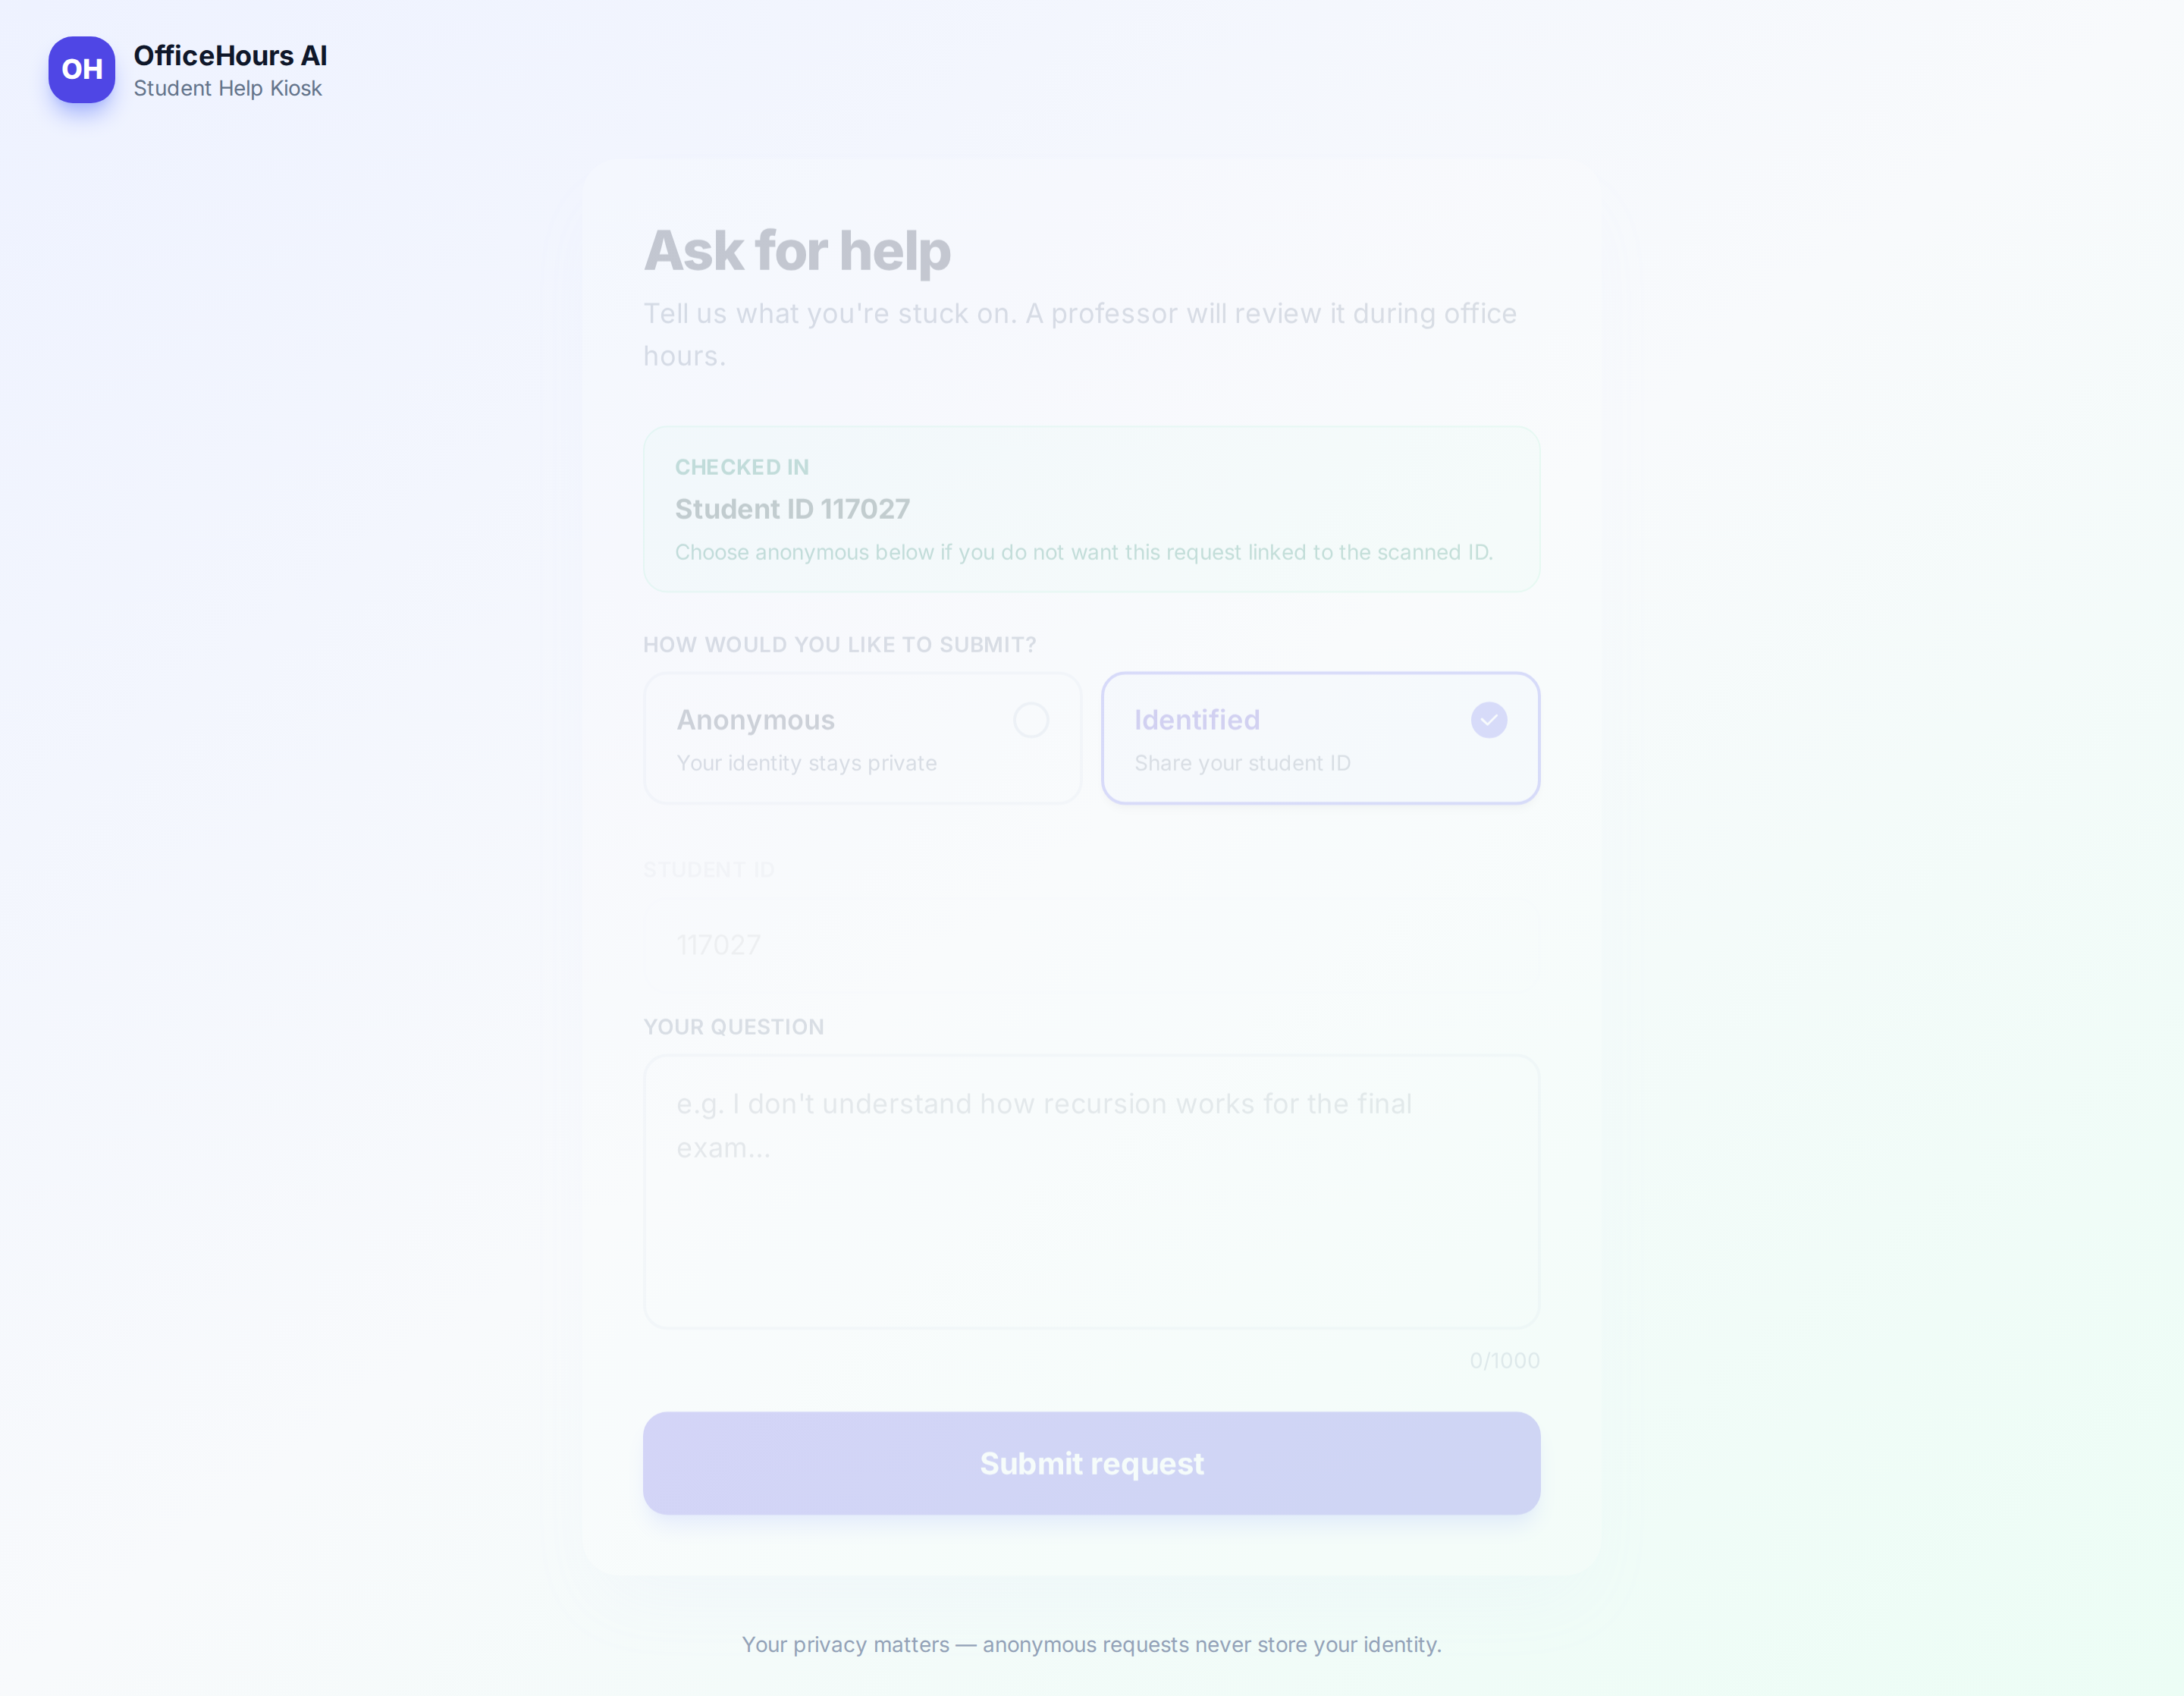
\includegraphics[width=0.92\linewidth]{../../demo/screenshots/02-student-request-form.png}
  \caption{Privacy-preserving request submission.}
\end{figure}

\begin{figure}[htbp]
  \centering
  
\includegraphics[width=0.85\linewidth]{../../demo/screenshots/05-recommendation-cards.png}
  \caption{AI-assisted recommendation cards.}
\end{figure}

\begin{figure}[htbp]
  \centering
  
\includegraphics[width=0.85\linewidth]{../../demo/screenshots/06-action-orchestration-plan.png}
  \caption{Action plan after professor approval.}
\end{figure}

\section{Reproducibility}
\begin{itemize}[noitemsep]
  \item Seed demo data: \path{backend/scripts/seed_demo_data.py}
  \item Capture screenshots: \path{demo/capture_screenshots.mjs}
  \item Analyze surveys: \path{backend/scripts/analyze_survey_responses.py}
  \item Run tests: \path{pytest} from \path{backend/}
\end{itemize}

\end{document}
